\documentclass[12pt, a4paper, oneside]{article}
%die Pakete werden hier durch den Include-Befehl separat eingelesen
\usepackage[utf8]{inputenc}
\usepackage{amsmath} % Mathematik-Pakete
\usepackage{amsfonts}
%\usepackage{mathptmx} %times new roman
%\usepackage[T1]{fontenc} %vollen Zeichensatz ]
\usepackage{amssymb}
\usepackage[ngerman]{babel}
\usepackage{graphicx}
\usepackage{microtype} %besserer Randausgleich
\usepackage{footnote}
\usepackage{blindtext}
\usepackage{etoolbox}
%\usepackage{makeidx}
%\usepackage{dsfont}
\usepackage{lettrine}%\usepackage{geometry}
%\usepackage{xcolor} % Für verschiedene Farben
\newcommand{\ricardo}[1]{\colorbox{ForestGreen}{\color{white}   \textsf{\textbf{Ricardo}}} \textcolor{ForestGreen}{#1}}
\usepackage[pdfborderstyle={/S/U/W 1}]{hyperref} % Für interaktive Refernzierung im PDF
\usepackage{csquotes}
\usepackage{acro}
\usepackage{hyperref} % Für interaktive Refernzierung im PDF
\usepackage[onehalfspacing]{setspace}%Zeilenabstand 1.5
% \usepackage{picins} % Das Umfließen einer Grafik im Text kann mit dem Paket PicIns erreicht werden.
%\usepackage{fontspec} 

%\usepackage[utf8]{inputenc}
\usepackage[ngerman]{babel}
\usepackage[top=2.5cm, bottom=2.5cm, left=2cm, right=3.5cm]{geometry}
\usepackage{bibgerm}
\usepackage{tabularx}
\usepackage{adjustbox}
\usepackage{cite}
\usepackage{blindtext}
\usepackage{epsfig}
\usepackage{longtable}
%\usepackage{showframe}
\usepackage{dcolumn}%benötigt für stargaze
\usepackage{here}%lädt das Paket zum Erzwinge n der Grafikposition
\usepackage{floatflt}%Bilder im Fließtext
%\usepackage{fontspec}
%\usepackage{fontenc}
\usepackage{dsfont}
%\setsansfont[Ligatures=TeX]{Arial}
%\renewcommand{\familydefault}{\sfdefault}
%\usepackage{times}
\usepackage{graphicx}
\usepackage{epstopdf}

\usepackage{xcolor}
\usepackage{listings}

\usepackage{lipsum}


\usepackage[T1]{fontenc}
\usepackage{lmodern}



\lstset{language=R}
\lstset{basicstyle=\ttfamily,
basicstyle=\small}
\lstset{literate=%
  {Ö}{{\"O}}1
  {Ä}{{\"A}}1
  {Ü}{{\"U}}1
  {ß}{{\ss}}1
  {ü}{{\"u}}1
  {ä}{{\"a}}1
  {ö}{{\"o}}1
}

\title{\textbf{Titel der Arbeit}}
\author{Miriam Lischke}

\setlength{\parindent}{0cm} %keine Einrückung
\linespread{1.5} 

\acsetup{first-style=short}
\newpage
\newpage
%Hier fängt die Deklarierung von Akronymen
%in alphabetischer Reihenfolge an
%auf Akronym im Text verweisen mittels \ac{ }
\DeclareAcronym{AIC}{
	short = AIC ,
	long  = \hspace*{22mm}Akaike-Informationskriterium ,
	tag = abbrev
}

\DeclareAcronym{BLES}{
	short = BLES ,
	long  = \hspace*{19mm}Bester Linearer Erwartungstreuer Schätzer ,
	tag = abbrev
}

\DeclareAcronym{c.p.}{
	short = c.p. ,
	long  = \hspace*{22mm}ceteris paribus ,
	tag = abbrev
}


\DeclareAcronym{u.i.v.}{
	short = u.i.v. ,
	long  = \hspace*{22mm}unabhängig und identisch verteilt ,
	tag = abbrev
}

\DeclareAcronym{KQS}{
	short = KQS ,
	long  = \hspace*{20mm}Kleinste-Quadrate-Schätzung ,
	tag = abbrev
}


\DeclareAcronym{VA}{
	short = VA ,
	long  = \hspace*{23mm}Varianzanalyse ,
	tag = abbrev
}


\newpage
\newpage
%in alphabetischer Reihenfolge

\newcounter{SeitenzahlSpeicher}
\begin{document}

 \thispagestyle{empty}
\begin{titlepage}
	 \thispagestyle{empty}
	% thispagestyle{empty} unterdrückt Seitenzahlen auf der gewünschten Seite
	\newfont{\smc}{cmcsc10 at 12pt}
%	\maketitle
	%Aufpassen mit fi: Fehlercode U+FB01
	%%%%%%%%%%%%%%%%%%%%%%%%%%%%%%%%%%%%%%%%%%
%Titel, Autor, Seminar, Semester, Dozent %
%%%%%%%%%%%%%%%%%%%%%%%%%%%%%%%%%%%%%%%%%%
\begin{center}
	 \thispagestyle{empty}
\begin{figure}[t]
	\centering
	
\includegraphics[width=0.6\textwidth]{assets/HTW_Logo.jpg}
	%\includegraphics[width=0.8\textwidth]{UniGoettingen.pdf}
	
\end{figure}

$~~$\\
\textbf{\huge Entwicklung eines Self-Service zur Bewertung digitaler Anwendung auf Verschreibungsfähigkeit }\paragraph{}$~~$\\
%\textbf{\huge Entwicklung eines Self-Service zur Feststellung des DiGA Status einer digitalen Anwendung}\paragraph{}$~~$\\
\paragraph{}$~~$\\
\paragraph{}$~~$\\
\textbf{Forschungsprojekt Teil B}\\ \textbf{an der Hochschule für Technik und Wirtschaft Berlin}
\paragraph{}$~~$\\
\paragraph{}$~~$\\
\paragraph{}$~~$\\
\text{vorgelegt am: \today}\\
\text{von: Miriam Lischke}\\
%\text{aus: Berlin}\\
\text{1. Gutachter: Prof. Dr. Peter Hufnagl}\\
\text{2. Gutachter: M Sc. Thorsten Knape}\\
\paragraph{}$~~$\\
%\text{Hochschule für Technik und Wirtschaft}\\
%\text{Professur für empirische Außenwirtschaft}\\
\end{center}	
\end{titlepage}



\begin{spacing}{1}
\pagenumbering{Roman}
\setcounter{page}{2}
\tableofcontents
\end{spacing}
\newpage
\begin{spacing}{1}
\section*{Abbildungsverzeichnis} 
\addcontentsline{toc}{section}{Abbildungsverzeichnis}
\renewcommand{\listfigurename}{}
\listoffigures
\end{spacing}
\newpage
\section*{Tabellenverzeichnis} 
\addcontentsline{toc}{section}{Tabellenverzeichnis} 
\renewcommand{\listtablename}{}
\listoftables % Tabellenverzeichnis
\footnote{Alle Tabellen wurden eigenständig erstellt, siehe \emph{R}-Code} 
%\newpage
%\section*{Symbolverzeichnis} 
%\addcontentsline{toc}{section}{Symbolverzeichnis} 
%Sortieren nach Auftreten im Text

%\begin{table}[h] \begin{center} \begin{tabular}{|lll|} \hline 
% & \textbf{Symbol} & \textbf{Bedeutung} \\ \hline \hline
% & $H_0 \colon$ &Nullhypothese\\ 
% & $H_1 \colon$ &Alternativhypothese\\
% & $\mathbf{I}_n\colon$ &Einheitsmatrix der Dimension $n$\\
% & $k$ &Anzahl der unabhängigen Variablen\\
% & $L(\cdot)$ &Plausibilitätsfunktion bzw. Likelihood-Funktion\\ 
% & $\ell(\cdot)$ & logarithmische Plausibilitätsfunktion bzw. log-Likelihood-Funktion\\ 
% & $n\colon$& Stichprobenumfang\\
% & $p$ &Anzahl der Regressionsparameter\\
% & $R^2\colon$ & Bestimmtheitsmaß\\ 
% & $\overline{R}^2\colon$ & adjustiertes Bestimmtheitsmaß\\ 
% & $\mathbf{X}\colon$& Versuchsplanmatrix \\ 
% & $\beta_1,\beta_2, \ldots, \beta_k\colon$& unbekannte Regressionsparameter\\ 
% & $ G_\Phi(\vartheta)$& Gütefunktion\\ 
% & $\hat{\boldsymbol \beta}\colon$& KQ-Schätzvektor \\ \hline
% \end{tabular} \end{center} \end{table}
%\newpage
%\section*{Abkürzungsverzeichnis} 
%\addcontentsline{toc}{section}{Abkürzungsverzeichnis}
%\printacronyms[include-classes=abbrev,name=Abkürzungen]
\newpage
\clearpage
\setcounter{SeitenzahlSpeicher}{\value{page}}
\pagenumbering{arabic}
\newpage
\pagenumbering{arabic}

\section{Einführung}
\subsection{Situationsbeschreibung}
\emph{Im Zuge der zunehmenden Digitalisierung} des Gesundheitswesens, ergeben sich für IT spezialisierte bzw. Unternehmen im Allgemeinen vermehrt Perspektiven in der Gesundheitsbranche fußzufassen. 
Aus diesen neuen Möglichkeiten der Branche entstehen eine Vielzahl an Kooperationen zwischen Experten aus verschiedensten Bereiche, wie etwa: Forschung, Wissenschaft, Public Health und Technologie etc. Dabei entstehen innovative Produkte, die dazu beitragen, das Gesundheitswesen voranzubringen. ``Mit dem Inkrafttreten des Digitale-Versorgung-Gesetzes (DVG) am 19. Dezember 2019 wurde die „App auf Rezept“ für Patientinnen und Patienten in die Gesundheitsversorgung eingeführt. 
Damit haben ca. 73 Millionen Versicherte in der gesetzlichen Krankenversicherung (GKV) einen Anspruch auf eine Versorgung mit digitalen Gesundheitsanwendungen (DiGA), die von Ärzten und Psychotherapeuten verordnet werden können und durch die Krankenkasse erstattet werden.''~\cite{leitfadenfasttrack}  
Dieser neue gesetzliche Rahmen schafft eine enorme Geschäftsnische für Unternehmen. 

Jedoch um für ein Produkt den offiziellen Status einer DiGA\footnote{Digitale Gesundheitsanwendung} zu erhalten muss mittels eines aufwendigen Prüfungsverfahren durch das Bundesinstitut für Arzneimittel und Medizinprodukte (BfArM), nach §139e SGB V ermittelt werden ob alle Voraussetzungen erfüllt sind. Erst nach erfolgreicher Prüfung erfolgt die Aufnahme in ein Verzeichnis für erstattungsfähige digitale Gesundheitsanwendungen (\textit{DiGA-Verzeichnis}~\cite{digaverzeichnis}) des BfArM\footnote{Bundesinstitut für Arzneimittel und Medizinprodukte\label{ftn:bfarm}}.

\subsection{Motivation und Forschungsfragen}
Das Verfahren nachdem das BfArM die potenzielle digitale Gesundheitsanwendung prüft nennt sich Fast-Track-Verfahren und wird durch einen Antrag zur Aufnahme in das DiGA-Verzeichnis angestoßen. Obwohl das Verfahren ``als zügiger ``Fast-Track'' (=schneller Weg) konzipiert''~\cite{digahersteller} ist, beträgt die Bearbeitungszeit drei Monate nach Eingang des vollständigen Antrags.

Zur Orientierung stellt das BfArM, den Antragssteller einen Umfangreichen Leitfaden gemäß § 139e Absatz 8 Satz 1 SGB V zur Verfügung. Dieser wendet sich in erster Linie an die Hersteller, denn die Anforderungen sind sehr hoch.

Der Leitfaden soll das Antragsverfahren in seinen Schritten übersichtlich darstellen und schafft Transparenz über die konkret zu erfüllenden Anforderungen im Verfahren und stellt sicher, dass alle Anträge nach gleichen Maßstäben bearbeitet werden.

Da der Leitfaden eher eine zusammenfassende Darstellung der
Regelungen, die an verschiedenen Stellen im SGB V\footnote{Sozialgesetzbuch, Fünftes Buch - Gesetzliche Krankenversicherung\label{ftn:sgb}}, in der DiGAV\footnote{Digitale-Gesundheitsanwendung-Verordnung\label{ftn:digav}} als auch in den Anlagen zur DiGAV zu finden sind, leistet und somit nur darlegt wie es die normativen Vorgaben aus DVG\footnote{Digitale-Versorgung-Gesetz\label{ftn:dvg}} und DiGAV regelmäßig auslegen.
Können vor allem junge Unternehmen wie Startups schnell den Überblick verlieren ob sie bereits die Voraussetzungen zur Antragsstellung erfüllen oder welche Schritte vorher noch eingeleitet werden müssen. Dies fordert viel Vorbereitung, Geld und Zeit. Da wäre es vom großen Vorteil mittels eines Vorabchecks zu prüfen ob bereits alle Anforderungen für einen erfolgreichen Ausgang der Antragsstellungen erfüllt sind oder in Form einer Roadmap aufweist welche Schritte dazu noch erforderlich sind. Daraus ergeben sich konkret die folgenden Forschungsfragen:
%Andererseits können all diese Anforderungen und zusammenfassenden Darstellungen der Reglungen, die unter anderem an verschiedenen Stellen im SGB V, in der DIGAV und in den Anlagen zur DIGAV zufinden sind vor allem junge Unternehmen wie Startups übervordern. 

%Zur Orientierung stellt das BfArM, den Antragssteller einen Umfangreichen Leitfaden gemäß § 139e Absatz 8 Satz 1 SGB V zur Verfügung, denn die Anforderungen an die Hersteller sind sehr hoch.
\begin{enumerate}
         \item Wie lässt sich aus Sicht des Herstellers, der Prozess zur Feststellung ob ein Potential, der eigenen digitalen Anwendung vorliegt als erstattungsfähigen DiGA eingestuft zu werden, vereinfachen?
         %Lasst sich mittels eines entwickelten digitalen Self-Service (sog. "Fast-Track-Checker"), die Vorbereitung zur Antragsstellung auf Aufnahme einer DIGA in das Verzeichnis, die durch das Fast-Track-Verfahren geprüft wird, für Antragssteller bzw. Hersteller vereinfachen?
         \item Wie kann man ein Self-Service verwirklichen, der zur Vereinfachung des Fast-Track-Verfahren bei trägt?
         %der durch den Self-Service entstehenden DiGA-Canvas, zu einer druckfähigen PDF generiert werden, sodass er für Hersteller zur Übersicht der aktuellen Situation und Hilfestellung für die folgenden Schritte dient?
\end{enumerate}

\subsection{Vorgehensweise}
Ziel dieser Forschungsarbeit ist es ein digitalen Self-Service zu entwickeln, der bei der Vorbereitung zum Antrag auf Aufnahme in das DiGA-Verzeichnis unterstützt und mithilfe eines DiGA-Canvas, die Anforderungen und Voraussetzungen kompakt zusammenfässt. Dabei wird ausgiebig erforscht, wie sich die Prüfung durch das Fast-Track-Verfahren zusammensetzt und welche Anforderungen sich dabei an die Hersteller und die Anwendung richten. Des Weiteren wird erforscht welche relevanten Informationen auf dem DiGA-Canvas zur Übersicht zusammengefasst werden sollten und mithilfe welcher Technologie, eine druckfähige PDF generiert werden kann.

\section{App auf Rezept}
Wie bereits erwähnt würde am 19.Dezember 2019 mit der Inkraftsetzung des Digitale-Versorgungs-Gesetzes (DVG), die ``App auf Rezept'' für Patientinnen und Patienten in die Gesundheitsverordnung eingeführt. Digitale Gesundheitsanwendungen (DiGA) können somit von Ärzten und Psychotherapeuten verordnet und durch die Krankenkasse erstattet werden. Dies eröffnet vielfältige Möglichkeiten, um bei der Erkennung und Behandlung von Krankheiten sowie auf dem Weg zu einer selbstbestimmten gesundheitsförderlichen Lebensführung zu unterstützen.

``Das BfArM hat diesen bedeutenden Baustein der Digitalisierungsstrategie der Bundesregierung und des Bundesgesundheitsministeriums von Anfang an mitgestaltet und unterstützt Hersteller und Anwender digitaler Medizinprodukte wie z.B. Medical Apps seit Jahren intensiv u.a. bei Fragen zur Einstufung einer App als Medizinprodukt oder zur Cybersicherheit von Medizinprodukten.'' /cite(https://diga.bfarm.de/de)

``Das Bundesinstitut für Arzneimittel und Medizinprodukte (BfArM) ist eine selbstständige Bundesoberbehörde im Geschäftsbereich des Bundesministeriums für Gesundheit (BMG). [... Es hat in diesem Kontext] die Aufgabe, Anträge zur Aufnahme von DiGA in das Verzeichnis wissenschaftlich zu bewerten. Es stellt außerdem das Verzeichnis für digitale Medizinprodukte bereit, die nach erfolgreicher Prüfung als erstattungsfähige digitale Gesundheitsanwendungen (DiGA) gelistet werden'' /cite(https://diga.bfarm.de/de)

Über sogenannte ``Bekanntmachungen'' im Bundesanzeiger, die erstmals am \textit{06.1.2020}~\cite{https://diga.bfarm.de/assets/documents/201006_BfArM_Bekanntmachung-DiGA-1.pdf} und zuletzt am \textit{29.12.2020}~\cite{https://diga.bfarm.de/assets/documents/201229_BfArM_Bekanntmachung-DiGA-2.pdf} erschienen sind, werden Informationen wie die Errichtung des Verzeichnisses für digitale Gesundheitsanwendungen (DiGA), die Bildung neuer Gruppen oder die Veränderung bestehender Gruppen im DiGA-Verzeichnis, die Aufnahme neuer DiGA im DiGA-Verzeichnis, die Streichung von DiGA aus dem DiGA-Verzeichnis veröffentlicht. Diese Veröffentlichung folgt vierteljährlich.

Für ärztliche oder psychotherapeutische Leistungserbringer eröffnet das Verzeichnis vielfältige Möglichkeiten, sich einen Überblick über verfügbare DiGA zu verschaffen, die möglicherweise für ihre Patienten infrage kommen könnten. Die im Verzeichnis aufgeführten Informationen sollen das gemeinsame aussuchen mit dem Patienten, unterstützen. Sodass die zur aktuellen Situation am besten geeignete DiGA verordnet werden kann.

\subsection{Wie kann eine DiGA verordnet werden?}

\begin{figure}[H]
	\centering
	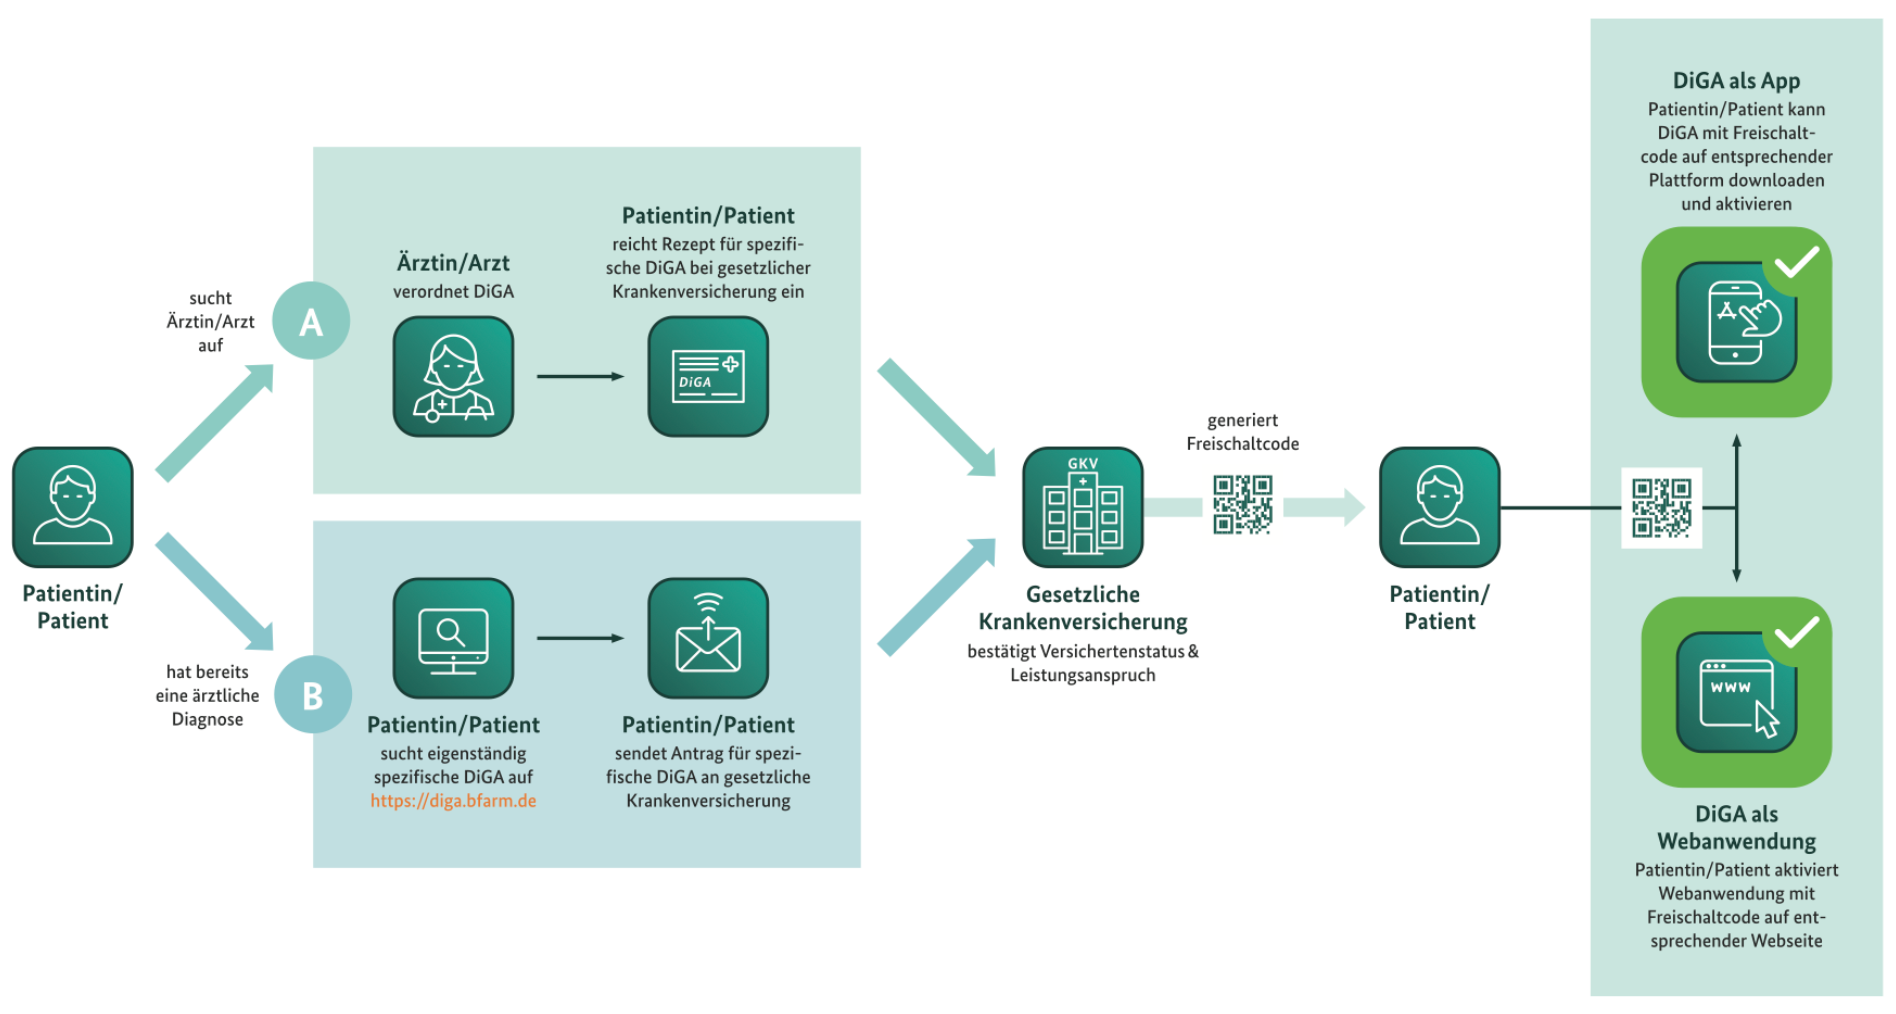
\includegraphics[width=450px, keepaspectratio]{assets/verordnungs_prozess.png}
	\caption{Graphauswertung - Komponentendiagramm,\\Quelle: Eigene Darstellung, Tool: \cite{visual_paradigm}}
\end{figure}
%Kern des Verfahrens sind die Prüfung der Herstellerangaben zu den geforderten Produkteigenschaften – vom Datenschutz bis zur Benutzerfreundlichkeit – sowie die Prüfung eines durch den Hersteller beizubringenden Nachweises für die mit der DiGA realisierbaren positiven Versorgungseffekte. Das sind Effekte, durch die sich der gesundheitliche Zustand eines Patienten oder die Möglichkeiten zum Umgang mit seiner Erkrankung durch die Benutzung der DiGA verbessern.
%
\begin{small}
\begin{quote}
"`Lorem ipsum dolor sit amet, consectetur adipisici elit, sed eiusmod tempor incidunt ut labore et dolore magna aliqua. Ut enim ad minim veniam, quis nostrud exercitation ullamco laboris nisi ut aliquid ex ea commodi consequat. Quis aute iure reprehenderit in voluptate velit esse cillum dolore eu fugiat nulla pariatur. Excepteur sint obcaecat cupiditat non proident, sunt in culpa qui officia deserunt mollit anim id est laborum."' (übersetzt durch Autor)\footnote{Bei Überzetzungen sollte genannt werden, ob es sich um eine in der Literatur rezipierte Übersetzung handelt, oder ob es sich um ein Eigenübersetzung des Autors handelt}
\end{quote}
\end{small}
%
Lorem ipsum dolor sit amet, consectetur adipisici elit, sed eiusmod tempor incidunt ut labore et dolore magna aliqua. Ut enim ad minim veniam, quis nostrud exercitation ullamco laboris nisi ut aliquid ex ea commodi consequat. Quis aute iure reprehenderit in voluptate velit esse cillum dolore eu fugiat nulla pariatur. Excepteur sint obcaecat cupiditat non proident, sunt in culpa qui officia deserunt mollit anim id est laborum.\\

\subsection{Wie funktioniert das Fast-Track- Verfahren?}

\begin{figure}[H]
	\centering
	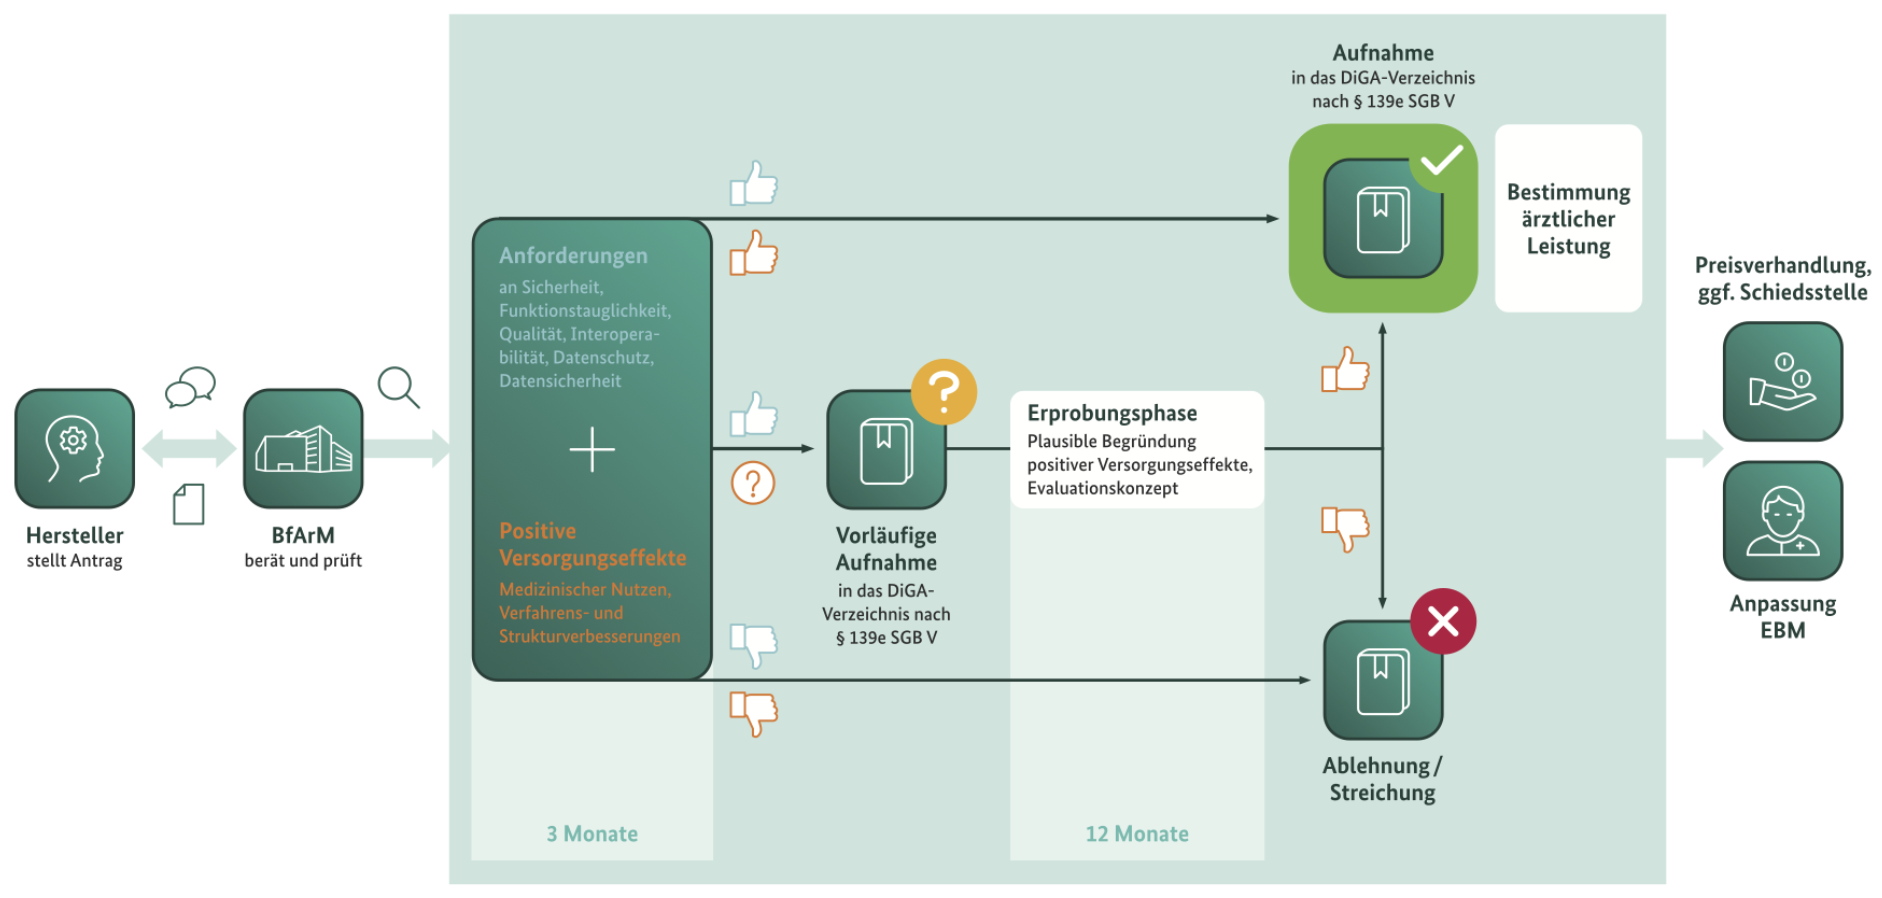
\includegraphics[width=450px, keepaspectratio]{assets/fastTrack_prozess.png}
	\caption{Graphauswertung - Komponentendiagramm,\\Quelle: Eigene Darstellung, Tool: \cite{visual_paradigm}}
\end{figure}
Lorem ipsum dolor sit amet, consectetur adipisici elit, sed eiusmod tempor incidunt ut labore et dolore magna aliqua. Ut enim ad minim veniam, quis nostrud exercitation ullamco laboris nisi ut aliquid ex ea commodi consequat. Quis aute iure reprehenderit in voluptate velit esse cillum dolore eu fugiat nulla pariatur. Excepteur sint obcaecat cupiditat non proident, sunt in culpa qui officia deserunt mollit anim id est laborum.

\subsection{Probleme bei der Analyse des Arbitrageverhaltens}
Lorem ipsum dolor sit amet, consectetur adipisici elit, sed eiusmod tempor incidunt ut labore et dolore magna aliqua. Ut enim ad minim veniam, quis nostrud exercitation ullamco laboris nisi ut aliquid ex ea commodi consequat. Quis aute iure reprehenderit in voluptate velit esse cillum dolore eu fugiat nulla pariatur. Excepteur sint obcaecat cupiditat non proident, sunt in culpa qui officia deserunt mollit anim id est laborum.\\
%
\begin{enumerate}
 \item Lorem ipsum
\item dolor sit amet, consectetur adipisici elit
\item sed eiusmod tempor incidunt ut labore et dolore magna aliqua
\end{enumerate}
%
Lorem ipsum dolor sit amet, consectetur adipisici elit, sed eiusmod tempor incidunt ut labore et dolore magna aliqua. Ut enim ad minim veniam, quis nostrud exercitation ullamco laboris nisi ut aliquid ex ea commodi consequat. Quis aute iure reprehenderit in voluptate velit esse cillum dolore eu fugiat nulla pariatur. Excepteur sint obcaecat cupiditat non proident, sunt in culpa qui officia deserunt mollit anim id est laborum.\footnote{Lorem ipsum dolor sit amet, consectetur adipisici elit, sed eiusmod tempor incidunt ut labore et dolore magna aliqua.} Lorem ipsum dolor sit amet, consectetur adipisici elit, sed eiusmod tempor incidunt ut labore et dolore magna aliqua. Ut enim ad minim veniam, quis nostrud exercitation ullamco laboris nisi ut aliquid ex ea commodi consequat. Quis aute iure reprehenderit in voluptate velit esse cillum dolore eu fugiat nulla pariatur. Excepteur sint obcaecat cupiditat non proident, sunt in culpa qui officia deserunt mollit anim id est laborum.
\section{Anforderung an die technische Lösung}
Im nachfolgendem Abschnitt wird auf die Verordnung über das Fast-Track Verfahren und die Anforderungen nach dem digitale Gesundheitsanwendungen bewertet und als Erstattungsfähig eingestuft werden, beleuchtet. Diese wird mithilfe eines zugrundeliegenden DiGA-Fast-Track-Canvas
% des "Platform Ecosystem Manager - Healthcare (PEMH) 
(Quelle: Knape2020) veranschaulicht.
\subsection{ Bewertungsgrundlage einer DiGA }
Die Digitale Gesundheitsanwenungen-Verordnung (DIGVA) vom 8. April 2020, gilt als Richtlinie und Bewertungsgrundlage des Fast-Track-Verfahrens. Das BfArM richtet sich ausschließlich nach diesen Vorgaben. Diese Verordnung ist für jeden einsehbar und somit eine hervorragende Grundlage für die Hersteller zur Vorbereitung auf den Antrag.
Die Verordnung gliedert sich in 9 Abschnitte, die schriftlich festlegen was eine DiGA\footnote{Digitale Gesundheitsanwendung} auszeichnet.
\begin{enumerate}
	\item \small{Antragsberechtigung und Antragsinhalte}
	\item \small{Anforderungen an Sicherheit, Funktionstauglichkeit, Datenschutz und Sicherheit sowie Qualität digitaler Gesundheitsanwendungen}
	\item \small{Anforderungen an den Nachweis positiver Versorgungseffekte}
	\item \small{Ergänzende Vorschriften für das Verwaltungsverfahren}
	\item \small{Inhalte und Veröffentlichung des Verzeichnisses für digitale Gesundheitsanwendungen nach § 139e Absatz 1 des Fünften Buches Sozialgesetzbuch}
	\item \small{Beratung durch das Bundesinstitut für Arzneimittel und Medizinprodukte}
	\item \small{Gebühren und Auslagen}
	\item \small{Schiedsverfahren}
	\item \small{Schlussbestimmungen}
\end{enumerate}

Jedoch ist sie in der Form des Bundesgesetzblattes verfasst, sodass sie nicht unbedingt leserfreundlich und für jeden auf Anhieb verständlich ist. Dafür stellt das BfArm\footnote{Bundesinstitut für Arzneimittel und Medizinprodukte\label{ftn:bfarm}} online einen Leitpfaden zur Verfügung. Dieser enthält alle Informationen rund um das Themas DiGA. Von Antragsstellung bis hin zur Aufnahme ins Verzeichnis. Dieser Leitfaden des Bundesinstitut für Arzneimittel und Medizinprodukte enthält sehr viele Informationen und ist mit seinen 141 Seiten nicht gerade übersichtlich und kompakt.

Wie wäre es deshalb einen übersichtlichen Canvas zu haben, der in einer überschaubaren Form Überblick über alle relevanten Anforderungen gibt? Genau das bietet der DiGA-Fast-Track-Canvas (Quelle: Knape2020).
%des "Platform Ecosystem Manager - Healthcare (PEMH) \cite{bibid} 
Hier würden bereits alle wichtigen Punkte der Verordnung in einer kompakten Form zusammen gefasst.
Der Canvas besteht ebenfalls aus neun Haupteilen und eine Kopfbereich, der Bezeichnung der DiGA, Medizinprodukt-Risikoklasse (nach MDR), Autor, Datum und Versionsnummer zusammenfasst. Die weiteren Bereiche befassen sich mit den tieferen Grundanforderungen des Verfahrens und dienen als äquivalent zu den Abschnitten in der Verordnung. Die Überschriften sind überwiegend als Fragestellungen formuliert, sodass schnell klar ist was hier ``gefragt'' ist.
%\renewcommand{\labelenumi}{\roman{enumi})}
\begin{enumerate}
	\item \textbf{Wie lautet die medizinische Zweckbestimmung Indikation? Kontradiktion? Patientengruppe?}
	\\In diesem Abschnitt legt der Hersteller die medizinischen Zweckbestimmungen da, die laut DIGAV §2 Absatz 2 nach medizinprodukterechtlichen Vorschriften gelten. Unter anderem soll hier auch auf die ``Patientengruppen eingegangen werden, für die positive Versorgungseffekte nach den §§ 8 und 9 nachgewiesen wurde oder, im Falle der vorläufigen Aufnahme, in dem Erprobungszeitraum nachgewiesen werden sollen.'' \cite{Verordnung}
	\item \textbf{Was unterstützt die digitale Anwendung?}
	\\In diesen Abschnitt geht es darum festzustellen ob die digitale Gesundheitsanwendung zur Erkennung, Behandlung, Überwachung, Linderung, Kompensierung einer Krankheit oder Behinderung dient. Oder ob es sich hierbei um Präventionsmaßnahmen handelt. Den würde die digitale Gesundheitsanwendung nur zur Primärprävention dienen, handelt es sich hier nicht um eine DiGA und würde im Antragsfall abgelehnt werden.
	\item \textbf{Wer sind die Nutzer der digitalen Anwendung?}
	\\Hier wird Primär, wie die Fragestellung eindeutig vorgibt aus das Nutzersegment eingegangen. Denn abzuklären ist, ob Es sich bei den Nutzer nur um Patienten oder auch um Ärzte und Therapeuten gemeinsam handelt oder nur um Leistungserbringer handelt. Denn im letzteren Fall würde es sich wieder nicht um eine DiGA handeln.
	\item \textbf{Worin besteht die digitale Hauptfunktionalität der Anwendung?}
	\\Die Hauptfunktionalität ist insofern wichtig, dass es sich bei auf eine digitale Technologie beruhen sollte. Sollte dies nicht der Fall sein kann diese Anwendung ebenfalls nicht in das DiGA Verzeichnis aufgenommen werden und würde bei der Antragsstellung keine Zustimmung bekommen.
	\item \textbf{Welche DiGA-Anforderungen erfüllt der Hersteller?}
	\\Als nächstes wird auf die DiGA-Anforderungen eingegangen, die den Hersteller der digitalen Gesundheitsanwendung betreffen. Dieser Anforderungen bezieht sich vor allem auf den Abschnitt 2 im DIGAV, der sich Anforderung an die Sicherheit, Funktionstauglichkeit,Datenschutz und -sicherheit sowie Qualität vorgibt. Hier wird im §7 die notwendige Nachweis durch Zertifikate benannt und in §9 die Darlegung positiver Versorgungseffekte erklärt. Sollte einer der Ökonomischen Nutzen in der Reduzierung von Kosten liegen, würde auch dieser Antrag von der BfArm eine Abgelehnung erhalten.
	\item \textbf{Welche DiGA-Anforderung erfüllt die digitale Anwendung?}
	\\Dieser Abschnitt bietet einen guten Überblick über die Grundfunktionen, die die digitale Gesundheitsanwendung grundsätzlich erfüllen sollte. Anforderungen an die Anwendung spiegelt dich im Verlauf der gesamten Verordnung in verschiedenster Form wieder und sollte deshalb direkt vor Antragsstellung durchweg mit "ja" beantwortet sein. 
	\item \textbf{Welches sind die nächsten Schritte des Herstellers?}
	\\ Hier entsteht nach erfolgreicher Beantwortung des Canvas ein Leitfaden, welches noch Notwendige Schritte vor der Einleitung des Antrages sind und sichert somit die Hersteller ab, nichts relevantes aus den Augen zu verlieren.
	\item \textbf{Gebühren und Auslagen für Hersteller}
	\\Dieser Bereich stützt sich auf den Abschnitt 7 der Verordnung und gibt einen Ausblick auf welche Kosten in welcher Form und Höhe während des Prozess zur Einstufung als erstattungsfähigen digitale Gesundheitsanwendung anfallen.
	\item \textbf{Marktzugang}
	\\Dieser Bereich bezieht sich auf weitere Informationen, die Anwendung Typisieren . Zum Beispiel unter welchen ICD-10-Code diese Anwendung fällt.
	
\end{enumerate}

Nach Bearbeitung dieses Canvas erhält man ein gutes Verständnis über die aktuellen Situation der eigenen digitalen Anwendung und welche Schritte noch nötig sind eine erstattungsfähige Anwendung zu werden. 
\begin{figure}[H]
	\centering
	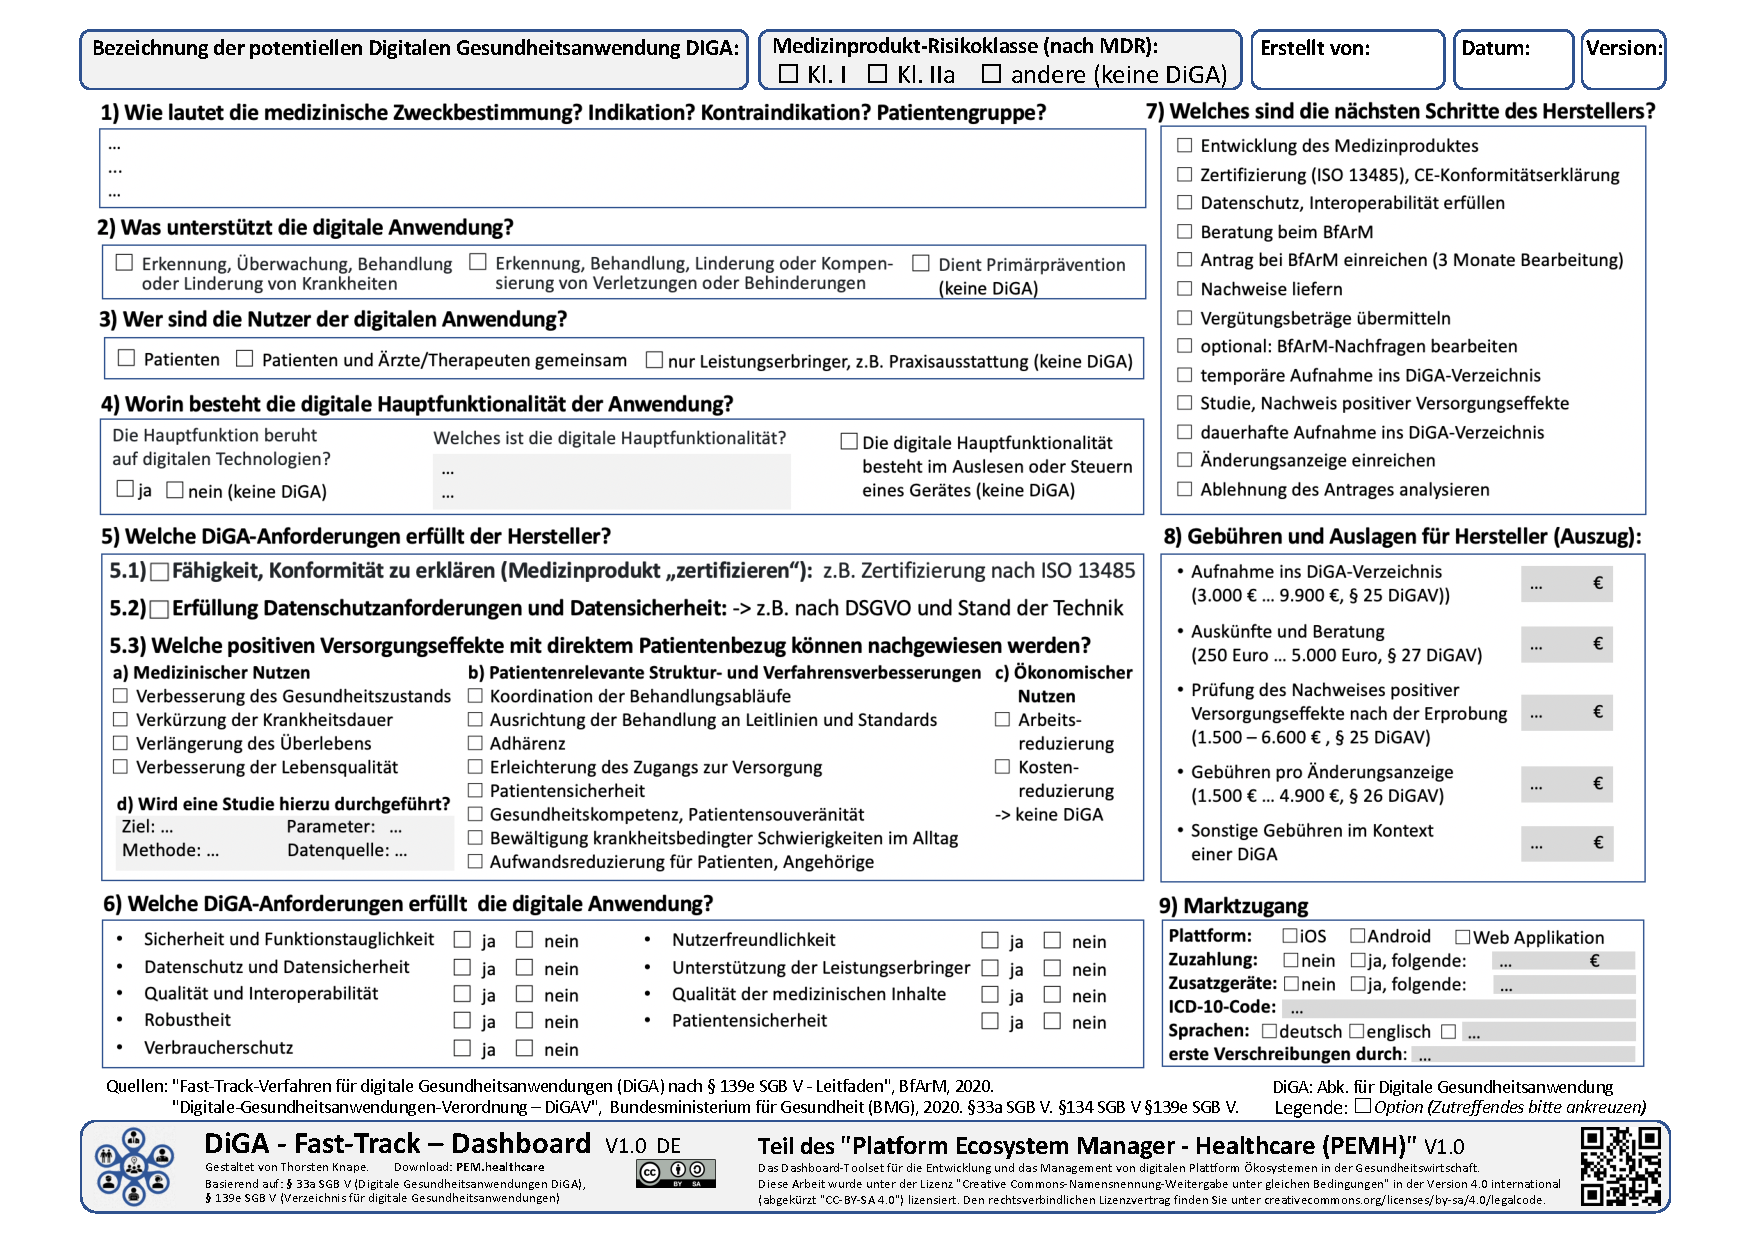
\includegraphics[width=450px, keepaspectratio]{assets/DiGA_Canvas.pdf}
	\caption[DiGA-Fast-Track-Canvas]{DiGA-Fast-Track-Canvas,~Quelle: Knape2020}
\end{figure}

Da die Anforderung an das Self-Service ist genau diese Klarheit zu schaffen, wird dieser Canvas als Grundlage für die Entwicklung des Tools dienen.

\subsection{Funktionale Anforderung des Self-Service}
Hauptfunktionalität des Self-Service wird es sein, eine Nutzeroberfläche für Hersteller anzubieten, in der Sie Angaben zu ihrer digitalen Gesundheitsanwendung machen.
Nach erfolgreichen befüllen werden die Antworten ausgewertet und einen Leitfaden über die nächsten Schritte ausgegeben. Die von dem Hersteller angegebenen Daten werden zusammen mit dem Leitfaden in einem Canvas zusammengefasst und können anschließend als PDF runter geladen werden.
\begin{figure}[H]
	\centering
	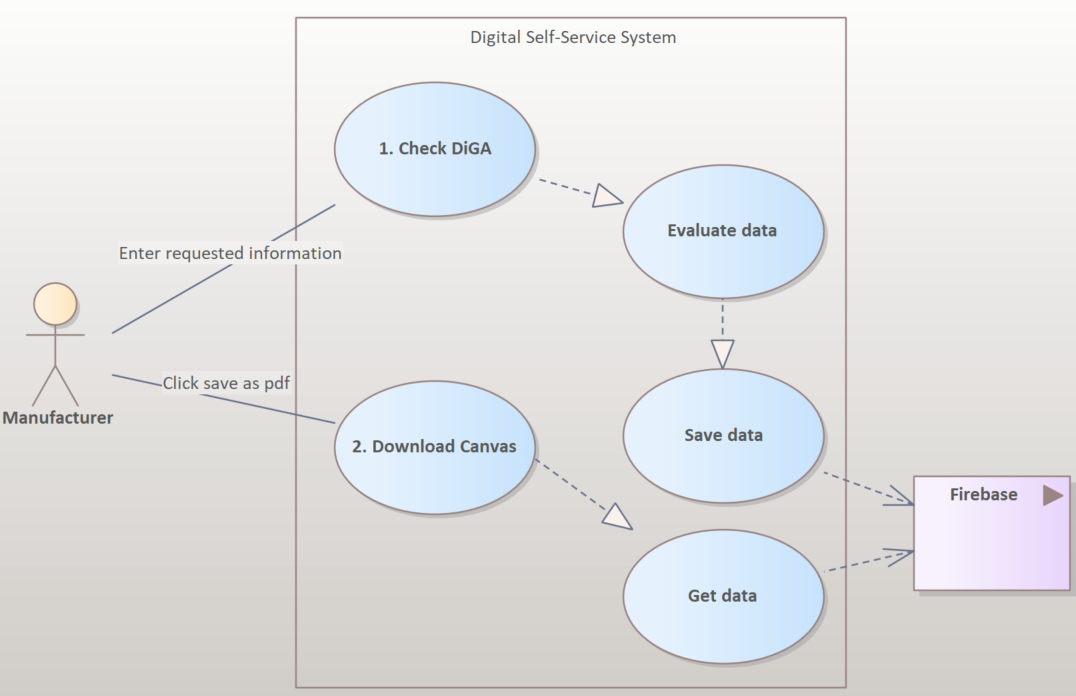
\includegraphics[width=450px, keepaspectratio]{assets/usecase1.png}
	\caption[Self-Service - Usecase Diagramm]{Self-Service - Usecase Diagramm,\\Quelle: Eigene Darstellung, Tool: \cite{enterpriseArchitect}}
\end{figure}

\section{Umsetzung des Self-Service}
Zur Umsetzung des Self-Service wurde das Framework~\textit{Angular 9}~\cite{angular} verwendet. Der gesamte Quellcode ist im GitHub-Repository \textit{MariamaB/tbc-app}~\cite{github_tbc} verfügbar. Mithilfe der~\textit{\textbf{N}ode \textbf{P}ackage \textbf{M}anager}~\cite{npm} (npm) und der Angular CLI wurde ein Angular Projekt aufgesetzt und alle weiteren packages installiert. Zudem wurden Hauptsächlich die Komponenten der ~\textit{Angular Material}~\cite{angularmaterial} Library verwendet um die UI zu entwickeln. Neben weiteren packages wurde~\textit{JsPDF}~\cite{jspdf} zur Generierung und Bereitstellung der PDF download Funktion eingesetzt.
\\\\
Die Nutzeroberfläche hat derzeit zwei Zustände. Im 1. Zustand hat der Nutzer die Möglichkeit die gefragten Informationen direkt ins Canvas einzugeben Abbildung~\ref{fig:canvasonedit}. Diese hätte auch mit einen Fragebogen gelöst werden können, jedoch bekommt der Nutzer so einen besseren Überblickt was noch gefragt ist und kann sich quasi die Reihenfolge der Bearbeitung nach belieben aussuchen. Außerdem kann so am Ende alles auf einem Blick gegen geprüft werden und bei Unzufriedenheit oder Unvollständigkeit nach gebessert werden.
\begin{figure}[H]
	\centering
	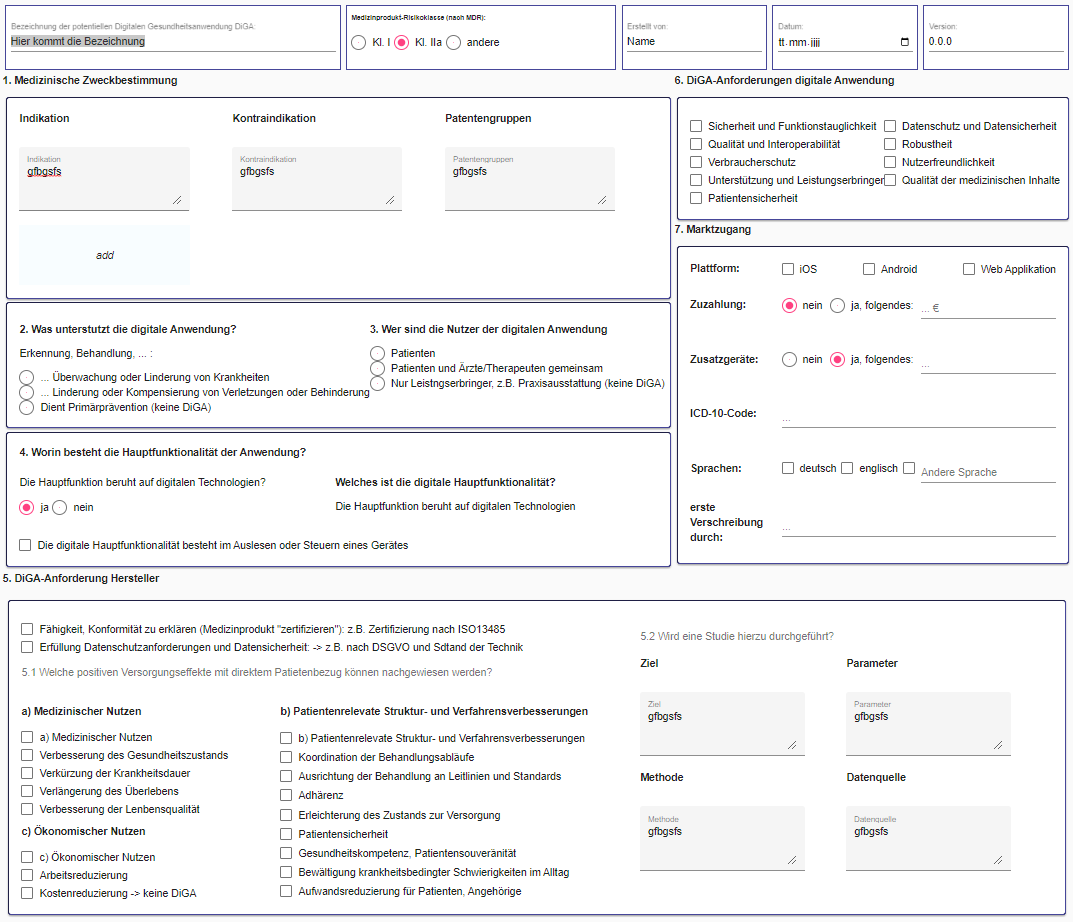
\includegraphics[width=350px, keepaspectratio]{assets/onEdit.png}
	\caption[DiGA-Canvas - Bearbeitungsmodus]{DiGA-Canvas - Bearbeitungsmodus,~Quelle: Eigene Entwicklung}
	\label{fig:canvasonedit}
\end{figure}
Der 2. Zustand ist die gespeicherte Version des Canvas Abbildung~\ref{fig:canvasonsave}. Zu diesem Status kommen zwei weitere Felder:
\begin{itemize}
	\item Welches sind die nächsten Schritte des Herstellers?
	\item Gebühren und Auslagen für Hersteller
\end{itemize}
 Das sind Felder, die von dem Self-Service zur Information des Herstellers nach Bearbeitung des Canvas ausgewertet und befüllt werden. Anschließend besteht die Option diesen Canvas in dieser Form als PDF zu downloaden.
  \begin{figure}[H]
  	\centering
  	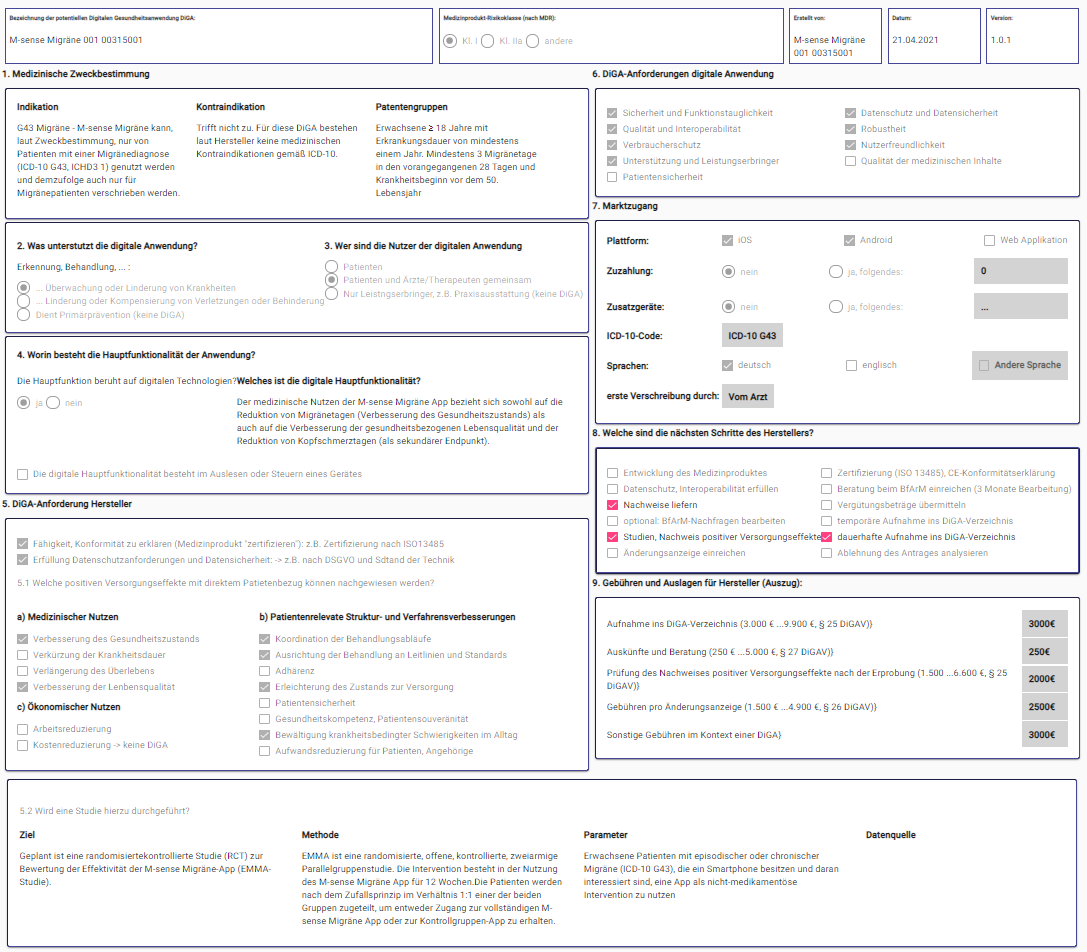
\includegraphics[width=350px, keepaspectratio]{assets/onSave.png}
  	\caption[DiGA-Canvas - Gespeicherter Modus]{DiGA-Canvas - Gespeicherter Modus,~Quelle: Eigene Entwicklung}
  	\label{fig:canvasonsave}
  \end{figure}
Als Background Komponente wird eine~\textit{Firebase}~\cite{firebase} Realtime Datenbank verwendet. In der alle eingegebenen und generierten Daten verwaltet werden. Mittels der~\textit{Angularfire}~\cite{angularfire} Library interagiert das Angular Projekt direkt mit der Firebase Datenbank. Über die Firebase Console lassen sich die Daten verwalten und einsehen.
  
    \begin{figure}[H]
  	\centering
  	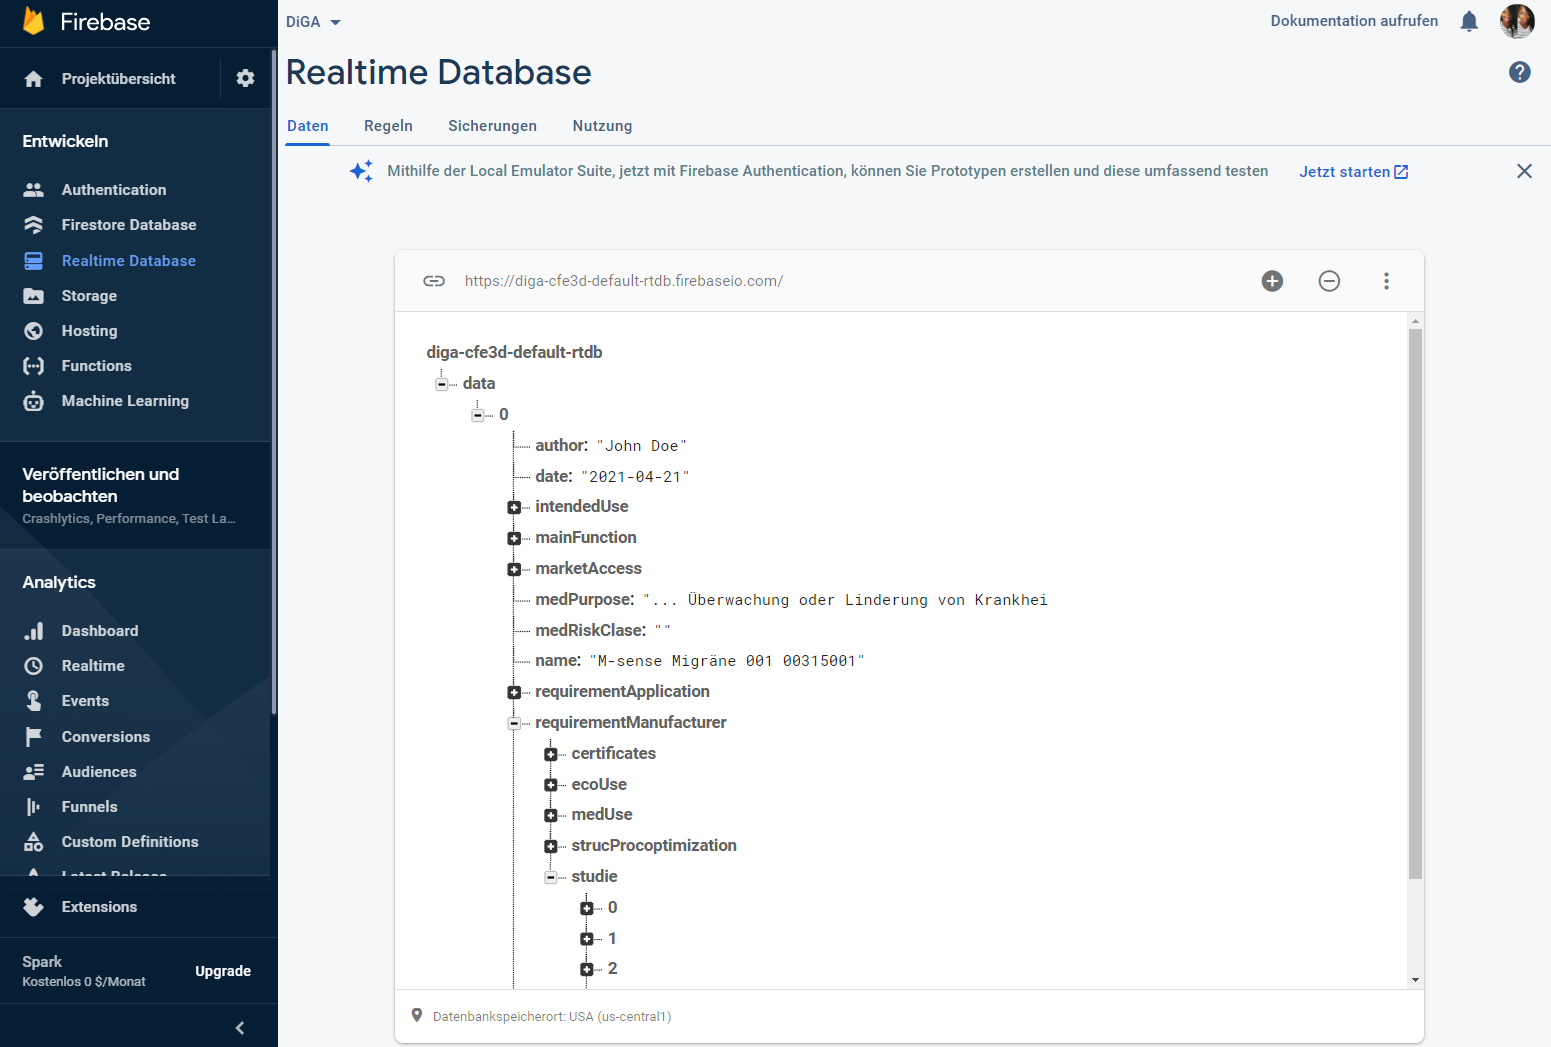
\includegraphics[width=350px, keepaspectratio]{assets/firebaseConsole.png}
  	\caption[Firebase Console - Realtime Database]{Firebase Console - Realtime Database,~Quelle:~\cite{firebase}}
  \end{figure}
\section{Kritische Betrachtung und Limitationen}
Die Bereitstellung eines Self-Service zur Überprüfung der eigenen zugrundeliegenden digitalen Gesundheitsanwendung ist eine praktische und übersichtliche Weise für Hersteller vor Antragsstellung eine Einschätzung einzuholen. So erhalten Sie in einer kompakten Form, die Auskunft ob sich der gesamte Aufwand lohnt. Das spart Zeit als auch Kosten, was vor allem kleinere Unternehmen sowie Startups sehr entgegen kommt. Allerdings handelt es sich hier nach erfolgreicher Bearbeitung des Canvas zu nächst nur um eine Momentaufnahme. Der Canvas verändert sich nicht mit den Fortschritten der App dynamisch mit. Interessant wäre es, wenn es sich bei dem Self-Service um eine Plattform handeln würde, auf der man sein Projekt zur DiGA verwaltet. Und somit die Hersteller bis zur Antragsstellung begleitet während man weitere Fortschritte dokumentieren kann. Zudem könnte diese Plattform während jeder Phase weitere Tipps und Tricks zur Verfügung stellen, die dabei helfen schneller das gewünschte Ziel zu erreichen.
\section{Fazit und Ausblick}
Das Ziel, das zur Anfang in Form von Forschungsfragen formuliert wurde, wurde weitgehend erreicht. Einen digitaler Canvas, gebettet in einem einfachen Self-Service, der alle Informationen zur Überprüfung einer digitalen Gesundheitsanwendungen auf Erstattungsfähigkeit enthält, wurde umgesetzt. Der Nutzer dieses Self-Service kann bereits eine erste Version des Canvas mit den eingegebenen Daten als pdf downloaden, jedoch ist das System an dieser Stelle noch nicht soweit eine Auswertung nach DIGAV Verordnung vorzunehmen. Einen Ausblick wäre es diese Funktionalität weiter auszubauen und die Qualität der generierten PDF zu optimieren.

\newpage
\clearpage
\pagenumbering{Roman}
\setcounter{page}{\theSeitenzahlSpeicher}
%\blindtext[3]


%mit Bibtex gearbeitet:
%Falls die Referenzen nicht funktionieren, mehrmals kompilieren mit F6 - F11 - F6 - F6 und dann F1 (Reihenfolge beachten) versuchen
%google scolar dann auf zitieren Bixtex klicken und copy paste
%thebibliography=Datei auf die Zugegriffen wird
%\large If you want to learn about linear and semiparametric regression, you should try \cite{Regression}, whereas \cite{Hobbit} will be disappointing in this context.


\section{Literaturverzeichnis}
\bibliographystyle{gerplain}
\renewcommand{\refname}{} 
\bibliography{bibba}

\newpage


\appendix %Anhang
\pagenumbering{arabic}
%

%
\newpage

\end{document}